\documentclass[11pt]{article}
\usepackage[margin=1in]{geometry}
\usepackage{amsmath,amssymb,amsthm,mathtools}
\usepackage{booktabs}
\usepackage{pgfplots}
\pgfplotsset{compat=1.16}
\usepackage[hidelinks]{hyperref}
\usepackage{url}
\emergencystretch=2em

\newtheorem{theorem}{Theorem}[section]
\newtheorem{proposition}[theorem]{Proposition}
\newtheorem{lemma}[theorem]{Lemma}
\newtheorem{corollary}[theorem]{Corollary}
\theoremstyle{definition}
\newtheorem{definition}[theorem]{Definition}
\theoremstyle{remark}
\newtheorem{remark}[theorem]{Remark}

\newcommand{\norm}[1]{\lVert #1\rVert}
\newcommand{\ip}[2]{\langle #1,#2\rangle}
\newcommand{\E}{\mathbb{E}}
\newcommand{\N}{\mathbb{N}}
\newcommand{\R}{\mathbb{R}}
\newcommand{\Lip}{\operatorname{Lip}}
\newcommand{\sd}{\mathbin{\triangle}}
\newcommand{\hE}{h_E}
\newcommand{\lz}{\operatorname{lz}}
\newcommand{\lcp}{\operatorname{lcp}}

\title{An explicit isoperimetric constant for Thompson's group $F$}
\author{[AUTHOR NAME]\thanks{The results, proofs and computer certificates in this note were found and
checked by Claude (Anthropic) agents working under the direction of [AUTHOR NAME]. The note has had
no human peer review.}}
\date{October 2026 (draft)}

\begin{document}
\maketitle

\begin{abstract}
The recent preprint \cite{OAI} proves that Thompson's group $F$ is nonamenable, by a finite
averaging argument driven by a Lipschitz self-map of the Hilbert unit ball with displacement bounded
away from zero; the argument is formalized in Lean. Neither the preprint nor the formalization gives
an explicit boundary constant or a constant for a prescribed generating set. We make the argument
explicit for the standard generators $x_0,x_1$. With
\[
  \hE(F)=\inf_{\emptyset\neq A\subset F\ \text{finite}}\frac{|x_0A\sd A|+|x_1A\sd A|}{|A|}
\]
(the Cheeger constant of the $4$-regular Cayley graph), we prove unconditionally that
$\hE(F)\ge 2.109\times10^{-19}$, and $\hE(F)\ge 2.466\times10^{-19}$ with a sharper word count.
If the closed unit ball of an infinite-dimensional Hilbert space admits a $k$-Lipschitz retraction
onto its sphere, then $\hE(F)\ge g(k)$ for an explicit function $g$; the value
$k_0(\ell^2)\le 28.99$ reported in the literature (we have not seen the original source) would give
$\hE(F)\ge 8.596\times10^{-9}$. The ingredients are a computer-assisted
evaluation of one separation constant ($\sigma(1/32)=1/256$), the Hilbert-space form of the
normalization estimate, and direct word-length bounds for the transports in Cannon--Floyd--Parry
normal form. This is a standard effectivization of \cite{OAI}; we add no new mechanism. The best
known upper bound is $\hE(F)<0.4996$ (Guba).
\end{abstract}

\section{Introduction}

Let $F$ be Thompson's group of increasing piecewise linear homeomorphisms of $[0,1]$ with dyadic
breakpoints and slopes in $2^{\mathbb Z}$. We write products as composition, $hg=h\circ g$, as in
\cite{OAI}, and use the standard generators
\begin{gather*}
x_0:\ [0,\tfrac12]\to[0,\tfrac14],\ [\tfrac12,\tfrac34]\to[\tfrac14,\tfrac12],\
[\tfrac34,1]\to[\tfrac12,1];\\
x_1=\mathrm{id}\text{ on }[0,\tfrac12],\ \text{a half-scale copy of $x_0$ on }[\tfrac12,1].
\end{gather*}
For a nonempty finite $A\subset F$ put $\eta_i(A)=|x_iA\sd A|/|A|$ ($i=0,1$). In the Cayley graph
with edges $g\sim x_i^{\pm1}g$, a $4$-regular graph, the number of edges leaving $A$ is
$\sum_{s\in\{x_0^{\pm1},x_1^{\pm1}\}}|sA\setminus A|=|x_0A\sd A|+|x_1A\sd A|$, because
$|x^{-1}A\setminus A|=|A\setminus xA|$ and $|xA\setminus A|=|A\setminus xA|$. So
\[
  \hE(F)=\inf_A\bigl(\eta_0(A)+\eta_1(A)\bigr)
\]
is the edge-isoperimetric (Cheeger) constant of this graph. The map $g\mapsto g^{-1}$ identifies the
graph with the right Cayley graph, so $\hE(F)$ equals the constant $\iota^*$ of
Guba~\cite{Guba2025}, which satisfies $\delta+\iota^*=4$ with $\delta$ the density.
By F{\o}lner's criterion, $F$ is nonamenable if and only if $\hE(F)>0$.

\begin{theorem}[unconditional]\label{thm:main}
For every nonempty finite $A\subset F$,
\[
  |x_0A\sd A|+|x_1A\sd A|\ \ge\ c_\star\,|A|,\qquad c_\star=2.1091\ldots\times10^{-19}.
\]
More precisely, $c_\star=(\kappa-4/D)/(4(1-1/D)\bar M)$ with $\kappa=(2\cdot 29621120)^{-2}$,
$D=2^{59}$ and $\bar M=\bar M(59)=329.5+2\cdot59/(2^{59}-1)$ given in closed form in Lemma~\ref{lem:avg}.
The sharper word count of Lemma~\ref{lem:F2sharp} gives $\hE(F)\ge 2.4666\times10^{-19}$
(Theorem~\ref{thm:sharp}).
\end{theorem}

\begin{theorem}[conditional on a retraction constant]\label{thm:cond}
Suppose that for some $k>1$ the closed unit ball $B$ of an infinite-dimensional real Hilbert space
admits a $k$-Lipschitz retraction onto its unit sphere. Then $\hE(F)\ge g(k)$, where
\[
 g(k)=\max_{m\ge1}\frac{\kappa_k-4\cdot2^{-m}}{4(1-2^{-m})\bar M(m)},\qquad
 \kappa_k=\Bigl(\frac{2}{k(k+2)}\Bigr)^{2},
\]
and $\bar M(m)$ is the explicit average word length of Lemma~\ref{lem:avg}. Values are in
Table~\ref{tab:g} and Figure~\ref{fig:g}; in particular $g(29)=8.5964\times10^{-9}$,
$g(32.26)=5.540\times10^{-9}$, and $g(28.99)=8.6085\times10^{-9}$.
\end{theorem}

The optimal retraction constant $k_0(H)$ of a Hilbert space is known to satisfy
$4.5\le k_0(H)\le 28.99\ldots$. Chaoha--Goebel--Termwuttipong~\cite{CGT} quote $4.5\ldots\le k_0(H)\le28.99\ldots$ as the
published estimates ``(see books and~\cite{BCF})''; Mahesh~\cite{Mahesh} quotes
$4.58\le k_0(\ell^2)\le 28.99$ citing Casini--Piasecki~\cite{CP} and~\cite{BCF}. The upper bound
may therefore come from~\cite{BCF} or from~\cite{CP}; we have read neither. \emph{We have not been able to read the full text
of~\cite{BCF}.} So we have not checked that the
bound there is a proved theorem rather than a numerical estimate, or how many digits it has. Since
all separable infinite-dimensional real Hilbert spaces are isometric to $\ell^2$, if the bound
holds as quoted then some retraction has constant $<29$, and Theorem~\ref{thm:cond} gives
$\hE(F)\ge g(29)=8.596\times10^{-9}$. We state this consequence only conditionally. The value
$32.26$ in Table~\ref{tab:g} is a value we could not trace to a checked source; it is included only
to show how sensitive $g$ is to $k$.

\begin{corollary}[spectral form]\label{cor:spec}
Let $\lambda_0$ be the bottom of the spectrum of the combinatorial Laplacian $4I-\mathcal A$ of
the Cayley graph above, and $\rho$ the spectral radius of simple random walk on it. Then
\[
  \lambda_0\ \ge\ 4-\sqrt{16-\hE^2}\ \ge\ \frac{\hE^2}{8}\ \ge\ 5.56\times10^{-39},
  \qquad \rho\ \le\ \sqrt{1-\hE^2/16}\ \le\ 1-1.39\times10^{-39},
\]
and, under the hypothesis of Theorem~\ref{thm:cond} with $k=29$, $\lambda_0\ge 9.23\times10^{-18}$.
\end{corollary}
\begin{proof}
For an infinite graph of degree $d$ with edge-isoperimetric constant $i$, Mohar~\cite{Mohar}
proved $\lambda_0\ge d-\sqrt{d^2-i^2}$ (see also Lyons--Peres~\cite{LP}, Ch.~6, for the form $\rho\le\sqrt{1-(i/d)^2}$); and $d-\sqrt{d^2-i^2}\ge i^2/(2d)$. Take $d=4$, and use
$\rho=1-\lambda_0/4$ for the simple random walk on a regular graph.
\end{proof}

\paragraph{Known upper bounds.}
Guba~\cite{Guba2004} showed that the density is at least $3$, so $\hE(F)\le1$. Belk and
Brown~\cite{BelkBrown} built finite sets with density tending to $3.5$, so $\hE(F)\le1/2$.
Guba~\cite{Guba2025} beat $3.5$ (density $>3.5004$), so $\hE(F)<0.4996$. Hence
\[
 2.1\times10^{-19}\ \le\ \hE(F)\ <\ 0.4996 ,
\]
a gap of about $61$ binary orders of magnitude (about $26$ under the retraction hypothesis).

\paragraph{What is and is not new.}
The proof is the argument of~\cite{OAI} with every constant tracked. We change three things, all
routine: (i) we use the Hilbert-space Lipschitz constant $1/\varepsilon$ for radial normalization
in place of the Banach-space constant $2/\varepsilon$ used in~\cite{OAI} and its Lean code
(Lemma~\ref{lem:norm}); (ii) we evaluate the one non-explicit constant of the Lean construction,
a curve-separation constant, by a certified computation (Proposition~\ref{prop:sigma});
(iii) we replace the finite set $S$ of affine transports in~\cite{OAI} by $\{x_0,x_1\}$, using
explicit normal-form words and averaging the transport errors instead of taking their maximum
(Sections~\ref{sec:variance} and~\ref{sec:words}). No step of~\cite{OAI} fails and needs a new
idea. The note's only contribution is that the constant is explicit: as far as we know it is the
first explicit positive lower bound for an isoperimetric constant of $F$.

\section{Two elementary inequalities}

\begin{lemma}[translation subadditivity]\label{lem:sub}
Let $A\subset F$ be finite and $w=s_1\cdots s_\ell$ a word in $x_0^{\pm1},x_1^{\pm1}$ with $n_0$
letters $x_0^{\pm1}$ and $n_1$ letters $x_1^{\pm1}$. Then
$|wA\sd A|\le n_0|x_0A\sd A|+n_1|x_1A\sd A|$.
\end{lemma}
\begin{proof}
$|ghA\sd A|\le|ghA\sd gA|+|gA\sd A|=|hA\sd A|+|gA\sd A|$, and $|x^{-1}A\sd A|=|A\sd xA|$.
Induct on $\ell$.
\end{proof}

For $\psi:F\to[-1,1]$ and $h\in F$, cancellation over $hA\cap A$ gives \cite[\S2.3]{OAI}
\begin{equation}\label{eq:transl}
  \Bigl|\E_A\psi(h\,\cdot)-\E_A\psi\Bigr|\le\frac{|hA\sd A|}{|A|},\qquad
  \E_A\psi=\frac1{|A|}\sum_{g\in A}\psi(g).
\end{equation}

\begin{lemma}[normalization in Hilbert space]\label{lem:norm}
In a real inner product space, for $x,y\neq0$,
\[
 \Bigl\|\frac{x}{\norm x}-\frac{y}{\norm y}\Bigr\|\le\frac{\norm{x-y}}{\sqrt{\norm x\norm y}} .
\]
Hence $x\mapsto -x/\norm x$ is $1/\varepsilon$-Lipschitz on $\{\norm x\ge\varepsilon\}$.
\end{lemma}
\begin{proof}
$\norm{x-y}^2-\norm x\norm y\,\bigl\|\tfrac{x}{\norm x}-\tfrac{y}{\norm y}\bigr\|^2
=\norm x^2+\norm y^2-2\norm x\norm y=(\norm x-\norm y)^2\ge0$.
(Equivalently, $x/\norm x=P_B(x/\varepsilon)$ for $\norm x\ge\varepsilon$, with $P_B$ the
nonexpansive nearest-point projection onto $B$; see~\cite{CGT}.)
\end{proof}

\begin{remark}[where this enters]\label{rem:where}
The appendix of~\cite{OAI} defines $f(x)=-G(x)/\norm{G(x)}$ with $\norm{G}\ge\rho/4$ on $B$, and
says ``normalization on vectors of norm at least $\rho/4$ is Lipschitz with constant at most
$8/\rho$''. In the Lean code this is \texttt{normalizeNeg\_lipschitz} in
\texttt{AnalyticNormalization.lean} (the bound $2/\varepsilon$, proved for an arbitrary real normed
space), used through \texttt{normalizedMap\_lipschitz} in \texttt{AnalyticConstruction.lean}, where
\texttt{displacementLipschitzConstant} $=2\Lip(G)/(\rho/4)$. The space there is
$H=L^2([0,1];\R^2)$, an inner product space, so Lemma~\ref{lem:norm} applies with
$\varepsilon=\rho/4$ and gives $\Lip(f)\le4\Lip(G)/\rho$, half the formalized constant. The
$2/\varepsilon$ bound is sharp in general normed spaces, which is presumably why the generic Lean
lemma uses it. We have not changed the Lean code; Lemma~\ref{lem:norm} is a two-line identity.
\end{remark}

\section{The averaged variance inequality}\label{sec:variance}

Let $H$ be a real Hilbert space with closed unit ball $B$, and let $f:B\to B$ satisfy
$\norm{f(x)-f(y)}\le L\norm{x-y}$ and $\norm{f(x)-x}\ge\delta>0$. Put $\kappa=(\delta/L)^2$.

\paragraph{Dyadic layout.}
Identify a binary word $w$ with the basic interval $[0.w,0.w+2^{-|w|}]$; then $I\cdot J$ is word
concatenation. Fix $m\ge1$, put $D=2^m$, $r=m+2$, and take the \emph{parents}
\[
  P_u=u01\qquad(u\in\{0,1\}^m),
\]
ordered lexicographically. These are internal basic intervals of length $2^{-r}$ with pairwise
positive gaps (between $u01$ and the next parent lies at least the interval $u1$). The descendants
are $P_u\cdot P_v=u01v01$. The \emph{reference pair} is $P_0=01=[\frac14,\frac12]$,
$Q_0=101=[\frac58,\frac34]$. The proof of~\cite{OAI} works for any $D$ internal, pairwise separated
basic parents and any separated internal reference pair, since only the transport lemma and
the covariance identity of~\cite[\S2.1]{OAI} are used. This layout and the averaged form below are not part of the Lean development, which uses the
cells of depth $2D$ (\texttt{IntervalFamily.lean}) and the $\max_{h\in S}$ form; only the analytic
map of Section~\ref{sec:map} is taken from the formalization. Let $p(T)$ be the recursive coloring of~\cite{OAI} for
the parents $(P_u)$. Let $X_I(g)$ ($g\in F$) be the color of the normalized restriction of
$gT^{(n)}$ to $I$, for $I$ in $\mathcal I=\{P_u\}\cup\{P_uP_v\}\cup\{P_0,Q_0\}$, at a level $n$
that is admissible for every group element used below.

\paragraph{Transports.}
For each separated pair $I<J$ in $\mathcal I\setminus\{P_0,Q_0\}$, let $\varphi_{I,J}\in F$ carry
$I$ affinely onto $P_0$ and $J$ onto $Q_0$ (transport lemma of~\cite[\S2.1]{OAI}; an explicit choice is in
Section~\ref{sec:words}). By covariance~\cite[\S2.1]{OAI}, $\ip{X_I(g)}{X_J(g)}=\ip{X_{P_0}(\varphi_{I,J}g)}{X_{Q_0}(\varphi_{I,J}g)}$,
so with $\alpha=\E_A\ip{X_{P_0}}{X_{Q_0}}$ and~\eqref{eq:transl},
\begin{equation}\label{eq:eps}
  \bigl|\E_A\ip{X_I}{X_J}-\alpha\bigr|\le\epsilon(I,J):=\frac{|\varphi_{I,J}A\sd A|}{|A|}.
\end{equation}

\paragraph{The weighted pair family.}
Let $\mathcal P_m$ be the multiset of pairs, indexed by a row $u\in\{0,1\}^m$, consisting of
\emph{siblings} $(uv,uv')$ for $v\ne v'$ (we write $uv$ for $P_uP_v$; weight $1$), \emph{parents}
$(P_w,P_{w'})$ for $w\ne w'$ (weight $1$), and \emph{mixed} pairs $(uv,P_x)$ for $v$ arbitrary and
$x\ne u$ (weight $2$). Ordered pairs are used throughout; each is transported in increasing order.
The total weight is $W_m=4D^2(D-1)$. Write $\overline{\epsilon}$ for the $\mathcal P_m$-weighted
average of $\epsilon(I,J)$.

\begin{proposition}\label{prop:var}
For every nonempty finite $A\subset F$,
\[
  \kappa\ \le\ \frac4D+4\Bigl(1-\frac1D\Bigr)\overline{\epsilon}.
\]
\end{proposition}
\begin{proof}
For $g\in A$ put $m(g)=\frac1D\sum_uX_{P_u}(g)$ and $z_u(g)=\frac1D\sum_vX_{uv}(g)$. The recursion
gives $X_{P_u}=f(z_u)$, so, as in the proof of the boundary proposition of~\cite[\S2.3]{OAI},
$\delta^2\le\frac{L^2}{D}\sum_u\norm{z_u-m}^2$ pointwise on $A$. Expand
$\norm{z_u-m}^2=\norm{z_u}^2+\norm m^2-2\ip{z_u}{m}$ into $D^{-2}$-weighted inner products of
colors. Diagonal terms are at most $1$; the $D$ nested mixed terms $\ip{X_{uv}}{X_{P_u}}$ are at
least $-1$. Every other term is a separated pair, and by~\eqref{eq:eps} its average lies within
$\epsilon(I,J)$ of $\alpha$. The $\alpha$-coefficients are $D(D-1)+D(D-1)-2D(D-1)=0$, so
\[
 \E_A\norm{z_u-m}^2\le\frac4D+\frac1{D^2}\Bigl[\sum_{v\ne v'}\epsilon(uv,uv')+\sum_{w\ne w'}\epsilon(P_w,P_{w'})
   +2\sum_{v}\sum_{x\ne u}\epsilon(uv,P_x)\Bigr].
\]
Average over $u$, multiply by $L^2$, and note that the bracket summed over $u$ has total weight
$W_m=4D^2(D-1)$: this gives $\delta^2/L^2\le 4/D+(W_m/D^3)\,\overline\epsilon$, and
$W_m/D^3=4(1-1/D)$.
\end{proof}

With $\max_{h\in S}$ in place of the average this is the boundary proposition of~\cite[\S2.3]{OAI}. Since a
maximum dominates an average, the averaged form is legitimate. It matters here because the
transport words have very different lengths.

\begin{corollary}\label{cor:x0x1}
Let $\bar n_i$ be the $\mathcal P_m$-weighted average of the number of letters $x_i^{\pm1}$ in a
word for $\varphi_{I,J}$, and let $\bar M\ge\max(\bar n_0,\bar n_1)$. If $\kappa>4/D$, then for
every nonempty finite $A$,
\[
  \eta_0(A)+\eta_1(A)\ \ge\ \frac{\kappa-4/D}{4(1-1/D)\,\bar M}.
\]
\end{corollary}
\begin{proof}
By Lemma~\ref{lem:sub}, $\epsilon(I,J)\le n_0(I,J)\eta_0+n_1(I,J)\eta_1$, so
$\overline\epsilon\le\bar n_0\eta_0+\bar n_1\eta_1\le\bar M(\eta_0+\eta_1)$. Apply
Proposition~\ref{prop:var}.
\end{proof}

\begin{remark}[pairing]\label{rem:pairing}
Each sibling term and each parent term in the expansion can be compared \emph{directly} with a
mixed term, through one transport between the two pairs, instead of comparing both with $\alpha$.
Then the error term is $2(1-1/D)\eta$ instead of $4(1-1/D)\eta$, while the diagonal and nested
remainder stays $4/D$. In the $S$-form of~\cite{OAI} this halves the constant (sketch; not used below):
$\max_{h\in S'}|hA\sd A|/|A|\ge(\kappa-4/D)/(2(1-1/D))$ for a suitable finite $S'$. In the
$\{x_0,x_1\}$-form the direct transport costs, via the reference pair, at most the sum of the two
reference transports. So with the word bounds used here the pairing gives nothing, and we do not
use it.
\end{remark}

\section{The displacement map: explicit constants}\label{sec:map}

\subsection{The construction of the preprint}
The appendix of~\cite{OAI} works in $H=L^2([0,1];\R^2)$. It uses the curve
$\gamma(t)=a(t)v(t)$ with $v(t)(w)=(\cos\theta(t)w,\sin\theta(t)w)$ and
\[
 a(t)=\begin{cases}t/8,&t\le2\\ \frac5{16}-\frac{(3-t)^2}{16},&2<t<3\\ \frac5{16},&t\ge3\end{cases}
 \qquad
 \theta(t)=\begin{cases}0,&t\le1\\ \frac{(t-1)^2}2,&1<t<2\\ t-\frac32,&t\ge2.\end{cases}
\]
In the Lean structure \texttt{RegularCurveData}, the tube radius is
$\rho=\min(1/1024,\sigma/8)$, where $\sigma$ is any positive number with
$\norm{\gamma(t)-\gamma(s)}\ge\sigma$ whenever $|t-s|\ge1/32$. The development obtains $\sigma$
through \texttt{Classical.choose} from a compactness proof, so the formalized constant is not
explicit. Everything else is explicit. (Lean files, all in \texttt{OAI/GroupTheory/Thompson/}:
\texttt{TubeRegularCurve}, \texttt{AnalyticCorrection}, \texttt{CorrectionLocal},
\texttt{AnalyticConstruction}, \texttt{AnalyticNormalization}.) The correction $G$ satisfies $\norm{G}\ge\rho/4$, $G(x)=x$
for $\norm x\ge1/2$, and is Lipschitz with
\[
 \Lip(G)\le\max\Bigl(1,\ 30+\frac7{4\rho}+3808\rho,\ 5+\frac7{8\rho}\Bigr)
 \qquad(\texttt{CorrectionData.lipschitzConstant}).
\]
Then $f=-G/\norm G$ has $\norm{f(x)-x}\ge\delta=1/2$.

\subsection{The separation constant}

\begin{proposition}\label{prop:sigma}
$\sigma(1/32):=\inf_{|t-s|\ge1/32}\norm{\gamma(t)-\gamma(s)}=1/256$.
\end{proposition}
\begin{proof}
Since $\ip{v(s)}{v(t)}=\operatorname{sinc}(\theta(t)-\theta(s))$,
\[
  \norm{\gamma(t)-\gamma(s)}^2=a_t^2+a_s^2-2a_ta_s\operatorname{sinc}(\theta_t-\theta_s)
  =(a_t-a_s)^2+2a_ta_s\bigl(1-\operatorname{sinc}(\theta_t-\theta_s)\bigr).
\]
For $s<t\le1$ the curve is the segment $(t/8)v(0)$, so the distance is $(t-s)/8$. This gives
$\sigma\le1/256$, with equality at $t-s=1/32$. For the lower bound take $s<t$, $t-s\ge1/32$, and
split into cases:
\begin{enumerate}
\item[(A1)] $t\le1$: the distance is $(t-s)/8\ge1/256$.
\item[(A2)] $s\le0<1<t$: here $a_s\le0<\frac18\le a_t$. With $\min\operatorname{sinc}\ge-0.2173$
  we get $\norm{\cdot}^2\ge(1-0.2173)a_t^2\ge0.7827/64$.
\item[(A3)] $0\le s<t\le2$: here $a$ is linear with slope $1/8$, $a_s,a_t\ge0$, and
  $1-\operatorname{sinc}\ge0$; so $\norm\cdot\ge(t-s)/8$.
\item[(A4)] $s\ge3$: here $\norm\cdot^2=2(\frac5{16})^2(1-\operatorname{sinc}(t-s))\ge
  2(\frac5{16})^2(1-\operatorname{sinc}\frac1{32})$, since $\operatorname{sinc}$ decreases on
  $[0,\pi]$ and $|\operatorname{sinc}|\le1/\pi<\operatorname{sinc}\frac1{32}$ beyond $\pi$.
\item[(A5)] $0\le s\le3<5<t$: here $\theta_t-\theta_s\ge t-3\ge2$, so $|\operatorname{sinc}|\le\frac12$
  and $\norm\cdot^2\ge a_t^2+a_s^2-a_ta_s\ge\frac34a_t^2=\frac{75}{1024}>\frac3{64}$.
\item[(A6)] $0\le s\le3$, $2<t\le5$: this region is compact, and we treat it by computer.
\end{enumerate}
Cases (A2), (A4), (A5) have margins $801$, $2.08$ and $3072$ over $(1/256)^2$; the
inequality $\operatorname{sinc}\ge-0.2173$ is checked on $[1,1/0.2173]$ by interval bisection
($161$ boxes), and outside that range it is trivial. In (A6) we use coordinates
$(s,h=t-s)$ with $h\ge1/32$ and run a branch-and-bound in Arb ball arithmetic (128-bit,
outward rounding). On each box, $a$ and $\theta$ are enclosed piece by piece. When $t\le2$ we use
the exact identity $a_t-a_s=h/8$. For $|q|\le1$ we use the alternating-series enclosure
$q^2/6-q^4/120\le1-\operatorname{sinc}q\le q^2/6$, and otherwise the Arb enclosure of
$1-\sin q/q$. A box is accepted when the enclosure of $\norm\cdot^2$ lies strictly above
$(1/256)^2$; $6462$ boxes are accepted, and the smallest certified lower bound is
$1.0039\cdot(1/256)^2$. Box endpoints are rationals, entered as Arb balls containing them.
\end{proof}

The certificate is \texttt{cert.py}, part [A]. An independent re-implementation in
\texttt{mpmath.iv} with a different region split (script \texttt{v1\_sigma.py}) agrees.

\subsection{The constant chain}
With $\sigma=1/256$, $\rho=\min(1/1024,1/2048)=1/2048$ and
\[
 \Lip(G)\le 30+\tfrac74\cdot2048+\tfrac{3808}{2048}=\frac{231415}{64}=3615.859375,
 \qquad \varepsilon=\frac\rho4=\frac1{8192}.
\]
By Lemma~\ref{lem:norm}, $L=\Lip(G)/\varepsilon=29621120$, against $59242240$ with $2/\varepsilon$.
Hence
\[
 \kappa=\Bigl(\frac{1/2}{29621120}\Bigr)^2=2.8493\times10^{-16}
 \qquad(\text{with }2/\varepsilon:\ 7.1232\times10^{-17}).
\]
Substituting $\sigma=1/256$ for the \texttt{Classical.choose} value is legitimate because every
Lean lemma downstream of \texttt{RegularCurveData} is proved for an arbitrary separation constant
satisfying the separation property, and Proposition~\ref{prop:sigma} supplies that property for
$1/256$. That proposition is computer-assisted and not formalized.

\subsection{Maps from retractions}
\begin{lemma}\label{lem:retr}
If $R:B\to S$ is a $k$-Lipschitz retraction, then $f=-R$ is $k$-Lipschitz on $B$ and
$\norm{f(x)-x}\ge 2/(k+2)$.
\end{lemma}
\begin{proof}
Let $t=\norm x$. For $x=0$, $\norm{R(0)}=1$. Otherwise put $y=x/t\in S$, so $R(y)=y$. Then
$\norm{R(x)+x}\ge\norm{y+x}-\norm{R(x)-R(y)}\ge(1+t)-k(1-t)$, and also
$\norm{R(x)+x}\ge1-t$. The maximum of these two lower bounds is at least its value $2/(k+2)$ at
$t=k/(k+2)$, where they cross.
\end{proof}
Thus $\kappa_k=(2/(k(k+2)))^2$, which gives Theorem~\ref{thm:cond} once Section~\ref{sec:words}
supplies $\bar M$.

\section{Transport words in \texorpdfstring{$x_0,x_1$}{x0, x1}}\label{sec:words}

\paragraph{Tree pairs and normal form.}
A finite rooted binary tree $T$ is identified with its set of leaves, a set of binary words whose
intervals tile $[0,1]$. Let $N$ be its number of carets, so it has $N+1$ leaves. For two trees with
the same $N$, let $(T_-\to T_+)\in F$ be the element mapping the $k$-th leaf interval of $T_-$
affinely onto the $k$-th leaf interval of $T_+$. Let $R_N$ be the right vine. Following
Cannon--Floyd--Parry~\cite[\S2]{CFP}, the \emph{exponent} $e_k$ of the $k$-th leaf
($0\le k\le N$) is the length of the maximal chain of left edges ending at that leaf whose edges
do not hang from the right spine; that is, an edge from a vertex $1^j$ is not counted. In our
convention $hg=h\circ g$, with $x_{j+1}=x_0^{-1}x_jx_0$,
\begin{equation}\label{eq:cfp}
 (R_N\to T)=x_0^{e_0}x_1^{e_1}\cdots x_N^{e_N}
 = x_0^{e_0}\,x_1^{e_1}\,x_0^{-1}x_1^{e_2}\,x_0^{-1}\cdots x_0^{-1}x_1^{e_n}\,x_0^{\,n-1},
\end{equation}
where $n=\max\{k\ge1:e_k>0\}$ (the telescoped word is $x_0^{e_0}$ if no such $k$ exists). The certificate
checks~\eqref{eq:cfp} in exact arithmetic on $400$ random trees with up to $9$ carets, by verifying
that the word maps every leaf of $R_N$ affinely onto the corresponding leaf of $T$. In the
proof below we only need that the final words transport the right intervals, and the certificate
checks this directly for every pair at $m\le3$, a sample at $m=4$, and random pairs with
$m\le64$. We call $P(T)$ the right-hand word in~\eqref{eq:cfp}. Then
$(T_-\to T_+)=P(T_+)P(T_-)^{-1}$, and we freely reduce the concatenation.

Two facts follow from the definition. First, every caret has exactly one left edge, and each left
edge lies in exactly one maximal left chain; the uncounted edges are those hanging from the $s$
spine vertices $1^0,\dots,1^{s-1}$, where $s$ is the depth of the last leaf $1^s$. Hence
\begin{equation}\label{eq:sum}
  \textstyle\sum_{k=0}^Ne_k=N-s .
\end{equation}
Second, $e_N=0$. The penultimate leaf is $1^{s-1}01^j$: if $j\ge1$ it ends in $1$, and if $j=0$
its only left edge hangs from $1^{s-1}$. Either way $e_{N-1}=0$, so $n\le N-2$.

\paragraph{The transport.}
For a pair $I<J$ in $\mathcal P_m$, let $T_{\rm dom}$ be the minimal tree having $I$ and $J$ as
leaves. Its internal vertices are exactly the proper prefixes of $I$ and $J$. Its leaves split into
a left gap (before $I$), a middle gap and a right gap. The reference tree
$\{00,01,100,101,11\}$ has gaps $\{00\},\{100\},\{11\}$. Let $T_{\rm ran}$ be obtained from it by
repeatedly splitting the last leaf of each gap until each gap has as many leaves as the
corresponding gap of $T_{\rm dom}$. Then $\varphi_{I,J}=(T_{\rm dom}\to T_{\rm ran})$ carries $I$
onto $01$ and $J$ onto $101$ affinely.

\begin{lemma}[(F1)]\label{lem:F1}
All three gaps of $T_{\rm dom}$ are nonempty, so no padding of $T_{\rm dom}$ is needed, and
\[ N(\varphi_{I,J})=|I|+|J|-\lcp(I,J)-1 .\]
\end{lemma}
\begin{proof}
The left gap is empty only if $I$ is the leftmost leaf $0^{|I|}$; the right gap is empty only if
$J=1^{|J|}$; the middle gap is empty only if $I$ and $J$ are adjacent. Our intervals are internal
and separated, so none of these happens. The proper prefixes of $I$ and $J$ number $|I|+|J|$
counted with multiplicity; the common ones are those of length $0,\dots,\lcp(I,J)$, and
$\lcp<\min(|I|,|J|)$ because the intervals are not nested. So there are $|I|+|J|-\lcp-1$ carets.
\end{proof}

\begin{lemma}[(F2)]\label{lem:F2}
Let $e^{\rm d}_0,e^{\rm r}_0$ be the leftmost exponents and $s_{\rm d},s_{\rm r}$ the depths of
the last leaves of $T_{\rm dom},T_{\rm ran}$, and $N=N(\varphi_{I,J})$. The freely reduced word
$w=P(T_{\rm ran})P(T_{\rm dom})^{-1}$ satisfies
\[
 n_1(w)\le(N-s_{\rm r}-e^{\rm r}_0)+(N-s_{\rm d}-e^{\rm d}_0),\qquad
 n_0(w)\le e^{\rm r}_0+e^{\rm d}_0+2N-6,
\]
with $e^{\rm d}_0=\lz(I)$, the number of leading zeros of $I$, and $1\le e^{\rm r}_0\le2$.
\end{lemma}
\begin{proof}
By~\eqref{eq:cfp}, $P(T)$ has $\sum_{k\ge1}e_k=N-s-e_0$ letters $x_1^{\pm1}$, by~\eqref{eq:sum}.
It has $e_0+2(n-1)$ letters $x_0^{\pm1}$ (or $e_0$ if $n=0$): $e_0$ leading ones, $n-1$ interior
$x_0^{-1}$, and the tail $x_0^{n-1}$. Write $a=n_{\rm r}-1$ and $b=n_{\rm d}-1$. In
$P(T_{\rm ran})P(T_{\rm dom})^{-1}$ the tail $x_0^{a}$ meets the head $x_0^{-b}$ and freely reduces
to $x_0^{a-b}$. The $x_0$-count is therefore at most
$e^{\rm r}_0+e^{\rm d}_0+a+b+|a-b|=e^{\rm r}_0+e^{\rm d}_0+2\max(a,b)\le e^{\rm r}_0+e^{\rm d}_0+2(N-3)$,
using $n\le N-2$; when $n=0$ the bound holds since $N\ge3$. The leftmost leaf of $T_{\rm dom}$ is
$0^{\lz(I)+1}$, and its left chain hangs from the root, so $e^{\rm d}_0=\lz(I)$. The leftmost leaf
of $T_{\rm ran}$ is $00$ or $000$.
\end{proof}

\begin{lemma}[(F2$'$), sharper]\label{lem:F2sharp}
Let $g=g(J)$ be the number of zeros in the word $J$. If $J$ ends in $1$ (true for every interval
of the layout), then
\[ n_0(w)\le 2N-2g+e^{\rm d}_0-2,\qquad n_1(w)\le 2N-g-3-e^{\rm d}_0 .\]
\end{lemma}
\begin{proof}
The leaves of $T_{\rm dom}$ to the right of $J$ are the words $J_{<i}1$ for the positions $i$ with
$J_i=0$; none of them is a prefix of $I$, because $I$ lies to the left of $J$. So the right gap has
$g$ leaves, $J$ has index $N-g$, and all of these leaves, and $J$ itself, end in $1$ and have
exponent $0$. In $T_{\rm ran}$ the leaves from index $N-g$ on are $101,110,1110,\dots,1^{g}0,1^{g+1}$ (for $g=1$: $101,11$),
all of exponent $0$, so $s_{\rm r}=g+1$. Hence $n_{\rm d},n_{\rm r}\le N-g-1$, and the proof of
Lemma~\ref{lem:F2} gives $n_0\le e_0^{\rm r}+e_0^{\rm d}+2(N-g-2)$ and
$n_1\le(N-g-1-e_0^{\rm r})+(N-s_{\rm d}-e_0^{\rm d})$. Finally use $1\le e_0^{\rm r}\le2$ and
$s_{\rm d}\ge1$.
\end{proof}

Lemma~\ref{lem:F2} is Lemma~\ref{lem:F2sharp} without the gain from the right gap (that is,
with $g=1$). Both are checked pointwise for every pair at $m\le4$ and for $8500$ random pairs at
$m\in\{8,16,24,40,64\}$ (certificate, part [C]). A separate implementation
(\texttt{v2\_words.py}) also checks Lemmas~\ref{lem:F1} and~\ref{lem:F2}, and another
(\texttt{r1\_F2sharp.py}) checks Lemmas~\ref{lem:F1} and~\ref{lem:F2sharp}.

\begin{lemma}[closed-form averages]\label{lem:avg}
Let $\lambda=\frac{D-1-m}{D-1}$, let $a_k=\#\{u:\lz(u01)\ge k\}$ (so $a_k=D2^{-k}$ for $k\le m$,
$a_{m+1}=1$, and $a_k=0$ beyond), and let
$E_P=\sum_{k=1}^{m+1}\bigl(1-\frac{(D-a_k)(D-a_k-1)}{D(D-1)}\bigr)$. The $\mathcal P_m$-averages of
$N$, $\lz(I)$ and $g(J)$ are
\[
 \bar N=\frac{11r}4-1-\lambda,\qquad \bar e_0=\frac{1+3E_P}4,\qquad \bar g=\frac{3m+4}4 .
\]
Consequently, by Lemma~\ref{lem:F2},
$\bar M(m)=\max(2\bar N+\bar e_0-4,\ 2\bar N-2)$, and by Lemma~\ref{lem:F2sharp},
$\bar M'(m)=\max(2\bar N-2\bar g+\bar e_0-2,\ 2\bar N-\bar g-3-\bar e_0)$, are admissible in
Corollary~\ref{cor:x0x1}.
\end{lemma}
\begin{proof}
By Lemma~\ref{lem:F1}: siblings $u01v01<u01v'01$ give $N=3r-1-\lcp(v,v')$; parents give
$N=2r-1-\lcp(w,w')$; mixed pairs give $N=3r-1-\lcp(u,x)$. For distinct uniform
$v,v'\in\{0,1\}^m$, $\E\lcp=\sum_{k=1}^m\Pr[\lcp\ge k]=\sum_k\frac{D2^{-k}-1}{D-1}=\lambda$; weight
the three cases $1:1:2$. For $\bar e_0$: the lower interval of a sibling pair is $u01\cdots$, with
$\E\lz=\sum_k a_k/D=1$. The lower of $P_w,P_{w'}$ is the lexicographically smaller one, and its
leading-zero count is the larger of the two, which has expectation $E_P$. A mixed pair is ordered
by comparing $u$ with $x$, with the same expectation. For $\bar g$: for distinct uniform
$w,w'$, the larger has a $1$ where the smaller has a $0$ at the first difference and is otherwise
identically distributed, so $\E z(\max)=(m-1)/2$, where $z$ counts zeros. The upper intervals are
$u01\max(v,v')01$ (siblings, $\E g=m+\frac32$), $\max(w,w')01$ (parents, $\frac{m+1}2$), and,
with probability $\frac12$ each, $x01$ or $u01v01$ with $u=\max$ (mixed, $\frac{3m+4}4$). The
weighted mean is $\frac{3m+4}4$.
\end{proof}

The certificate compares all three closed forms with exhaustive enumeration for $m\le4$ (equality
of rationals). For instance $\bar M(59)=329.5+2(1-\lambda)$, i.e.\ $329.5$ up to $2\times10^{-16}$, and
$\bar M'(59)=281.75$. The exact averages $\bar n_0,\bar n_1$ at $m\le6$ lie well below both
bounds: at $m=6$ they are $28.15$ and $27.72$, against $\bar M=38.19$ and $\bar M'=30.18$. Extrapolating the
growth rates (about $4.55$ per unit of $m$ for $\bar n_1$, against $4.75$ for $\bar M'$) suggests that
exact counts would gain only about a further $5\%$ at $m=59$; we do not use this.

\section{Proofs of the theorems}

\begin{proof}[Proof of Theorem~\ref{thm:main}]
Take $f$ from Section~\ref{sec:map} with $\delta=1/2$ and $L=29621120$, so $\kappa=2.8493\times10^{-16}$.
In Corollary~\ref{cor:x0x1} take $\bar M=\bar M(m)$ and maximize over $m$; the maximum is at
$m=59$. The resulting exact rational is $c_\star=2.10918\ldots\times10^{-19}$ (Arb).
\end{proof}

\begin{theorem}\label{thm:sharp}
With $\bar M'(m)$ in place of $\bar M(m)$, $\hE(F)\ge2.4666\times10^{-19}$ (at $m=59$), and under the
hypothesis of Theorem~\ref{thm:cond}, $\hE(F)\ge g'(k)$ with $g'(29)=1.0197\times10^{-8}$.
\end{theorem}
\noindent
Lemma~\ref{lem:F2sharp} is proved here, checked by the certificate, and independently re-checked
(exhaustively for $m\le6$, on random pairs up to $m=100$, with whole-map transport checks).
The bounds of Lemma~\ref{lem:F2sharp} are attained for some pairs.

\begin{proof}[Proof of Theorem~\ref{thm:cond}]
Lemma~\ref{lem:retr} and Corollary~\ref{cor:x0x1} with $\bar M(m)$.
\end{proof}

\begin{table}[t]
\centering
\begin{tabular}{rcccc}
\toprule
$k$ & $\kappa_k$ & optimal $m$ & $\bar M(m)$ & $g(k)$\ \ [$g'(k)$ with $\bar M'$]\\
\midrule
3     & $1.78\times10^{-2}$ & 11 & 65.51  & $6.042\times10^{-5}$\ \ [$7.362\times10^{-5}$]\\
4.58  & $4.40\times10^{-3}$ & 13 & 76.50  & $1.280\times10^{-5}$\ \ [$1.548\times10^{-5}$]\\
6     & $1.74\times10^{-3}$ & 15 & 87.50  & $4.612\times10^{-6}$\ \ [$5.547\times10^{-6}$]\\
10    & $2.78\times10^{-4}$ & 18 & 104.0  & $6.311\times10^{-7}$\ \ [$7.544\times10^{-7}$]\\
20    & $2.07\times10^{-5}$ & 22 & 126.0  & $3.910\times10^{-8}$\ \ [$4.648\times10^{-8}$]\\
28.99 & $4.956\times10^{-6}$ & 24 & 137.0  & $8.6085\times10^{-9}$\ \ [$1.0211\times10^{-8}$]\\
29    & $4.949\times10^{-6}$ & 24 & 137.0  & $8.5964\times10^{-9}$\ \ [$1.0197\times10^{-8}$]\\
32.26 & $3.275\times10^{-6}$ & 24 & 137.0  & $5.540\times10^{-9}$\ \ [$6.572\times10^{-9}$]\\
33    & $2.998\times10^{-6}$ & 25 & 142.5  & $5.051\times10^{-9}$\ \ [$5.986\times10^{-9}$]\\
50    & $5.92\times10^{-7}$ & 27 & 153.5  & $9.152\times10^{-10}$\ \ [$1.083\times10^{-9}$]\\
100   & $3.84\times10^{-8}$ & 31 & 175.5  & $5.211\times10^{-11}$\ \ [$6.149\times10^{-11}$]\\
\bottomrule
\end{tabular}
\caption{The conditional bound $g(k)$ of Theorem~\ref{thm:cond}; in brackets, $g'(k)$ from
Theorem~\ref{thm:sharp}. Lower bounds for $k_0(H)$: $4.5$~\cite{CGT}, $4.58$~\cite{CP} (quoted in~\cite{Mahesh}).
Upper bound: $28.99$, quoted from~\cite{CP,BCF} (neither read by us).}
\label{tab:g}
\end{table}

\begin{figure}[t]
\centering
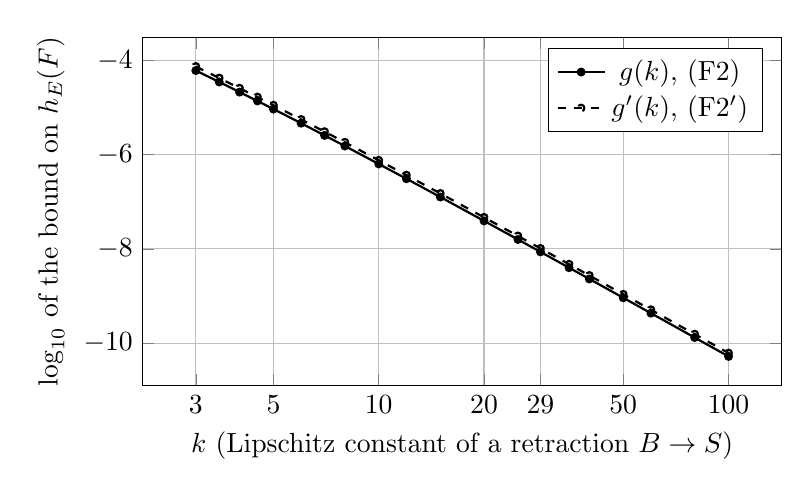
\begin{tikzpicture}
\begin{axis}[width=0.8\textwidth,height=6cm,xmode=log,xlabel={$k$ (Lipschitz constant of a retraction $B\to S$)},
 ylabel={$\log_{10}$ of the bound on $h_E(F)$},grid=major,legend pos=north east,
 xtick={3,5,10,20,29,50,100},xticklabels={3,5,10,20,29,50,100}]
\addplot[thick,mark=*,mark size=1.2pt] coordinates {(3,-4.2188) (3.5,-4.4612) (4,-4.6757) (4.5,-4.8638) (5,-5.0357) (6,-5.3361) (7,-5.5943) (8,-5.8193) (10,-6.1999) (12,-6.5141) (15,-6.9016) (20,-7.4078) (25,-7.8018) (29,-8.0657) (35,-8.4006) (40,-8.6395) (50,-9.0385) (60,-9.3655) (80,-9.8820) (100,-10.2830)};
\addlegendentry{$g(k)$, (F2)}
\addplot[thick,dashed,mark=o,mark size=1.2pt] coordinates {(3,-4.1330) (3.5,-4.3771) (4,-4.5931) (4.5,-4.7812) (5,-4.9544) (6,-5.2560) (7,-5.5151) (8,-5.7401) (10,-6.1224) (12,-6.4373) (15,-6.8254) (20,-7.3327) (25,-7.7272) (29,-7.9915) (35,-8.3269) (40,-8.5662) (50,-8.9655) (60,-9.2928) (80,-9.8099) (100,-10.2112)};
\addlegendentry{$g'(k)$, (F2$'$)}
\end{axis}
\end{tikzpicture}
\caption{Conditional lower bounds as functions of the retraction constant. For comparison, the
unconditional bound is $\log_{10}c_\star=-18.68$.}
\label{fig:g}
\end{figure}

\section{Where the constant was lost, and the limits of the method}

\begin{table}[t]
\centering
\begin{tabular}{lrl}
\toprule
factor & $\log_2$ & origin\\
\midrule
$\delta^2=1/4$ & $-2.00$ & displacement of $f=-G/\norm G$\\
$\varepsilon^2=(\rho/4)^2$, $\rho=1/2048$ & $-26.00$ & $\rho=\sigma/8$, $\sigma=\frac1{256}=\frac18\cdot\frac1{32}$ (speed $\times$ scale)\\
\quad [with $2/\varepsilon$ as in Lean] & [$-28.00$] & Banach-space normalization constant\\
$\Lip(G)^{-2}$, $\Lip(G)=3615.86$ & $-23.64$ & dominated by the cutoff term $7/(4\rho)=3584$\\
\midrule
$\kappa=(\delta/L)^2$ & $-51.64$ & \\
$(1-4/(D\kappa))/(4(1-1/D))$ & $-2.04$ & variance constant $4$; $D=2^{59}$\\
$1/\bar M$, $\bar M=329.5$ & $-8.36$ & word length of transports, $\approx5.5m$\\
\midrule
$\hE\ge c_\star$ & $-62.04$ & ($-61.81$ with (F2$'$), $-64.09$ with $2/\varepsilon$)\\
\bottomrule
\end{tabular}
\caption{Ledger for Theorem~\ref{thm:main}.}
\label{tab:ledger}
\end{table}

Table~\ref{tab:ledger} itemizes the loss. About $52$ of the $62$ binary orders come from the
analytic map: the squared ratio $(\delta/L)^2$ with $L\approx 7/\rho^2\approx2^{24.8}$. This in
turn comes from the tube radius $\rho=1/2048$, set by the slow speed $1/8$ of the curve, the
separation scale $1/32$, and the safety factor $8$ in $\rho=\sigma/8$. The group-theoretic part,
from the transports, costs about $10$ binary orders, of which $8.4$ are the average word length;
it is the only part that depends on $F$.

\paragraph{Ceilings.}
(i) For every $L$-Lipschitz $f:B\to B$ the minimal displacement is at most $1-1/L$ (Goebel; see
\cite{BWW}), so $\delta/L\le1/4$ and $\kappa\le1/16$. Inserted into Corollary~\ref{cor:x0x1}
with the present layout, this caps the method at $\hE\ge G(1/16)=2.51\times10^{-4}$ ($m=9$). In
the $S$-form of~\cite{OAI} the cap is $\kappa/4\le1/64$ for $\max_{h\in S}|hA\sd A|/|A|$.
(ii) Under the retraction hypothesis, $\kappa_k\le(2/15)^2$ at $k=3$, the universal lower bound
for $k_0$, so $g(k)\le g(3)=6.04\times10^{-5}$. (iii) As long as each pair is compared with a
reference pair through a single transport, the average word length grows linearly in $m$, while
$m\ge\log_2(4/\kappa)$ is forced. So the $\{x_0,x_1\}$-form always loses a factor of order
$\log(1/\kappa)$ relative to the $S$-form. Compared with the known upper bound $0.4996$, even
ceiling (i) is about $11$ binary orders short.

\paragraph{How one could do better.}
The real leverage is in $\kappa$. A different curve (faster speed, larger separation scale), or a
Lipschitz map with better displacement-to-Lipschitz ratio in Hilbert space, would help most;
under the retraction hypothesis this is the passage from $2.1\times10^{-19}$ to
$8.6\times10^{-9}$. On the group side, exact word counts (rather than the bounds of
Lemmas~\ref{lem:F2}--\ref{lem:F2sharp}) and better reference pairs could each gain a constant
factor. We have not pursued these.

\section*{Reproducibility}
\texttt{cert.py} (Python 3, \texttt{python-flint} 0.9) recomputes, in about 15 seconds on one core:
[A] Proposition~\ref{prop:sigma}; [B] the constant chain, in exact rationals; [C] the word-length
facts and closed forms (exhaustive for $m\le4$, random up to $m=64$, including the transport
property of the words); [D] all bounds in Theorems~\ref{thm:main}, \ref{thm:cond},
\ref{thm:sharp} and Table~\ref{tab:g}, as exact rationals printed through Arb; [E] the ceilings,
the ledger and Corollary~\ref{cor:spec}. Its output is saved as \texttt{cert\_output.txt}.
Separately written scripts check the same ingredients:
\texttt{s1\_sigma\_paper\_curve.py} and \texttt{v1\_sigma.py} (the latter in \texttt{mpmath.iv}) check
Proposition~\ref{prop:sigma}; \texttt{s4\_wordlength\_R.py}, \texttt{v2\_words.py} and
\texttt{v3\_avg.py} check (F1), (F2) and the closed forms; and \texttt{v4\_constants.py}
reproduces the (F2)-based values $2.1092\times10^{-19}$, $5.1026\times10^{-20}$ and
$8.5964\times10^{-9}$; \texttt{r1\_F2sharp.py} checks (F1), (F2$'$), the closed-form averages and the
transport property with its own data structures.

\begin{thebibliography}{99}
\bibitem{OAI} OpenAI, \emph{Thompson's group $F$ is nonamenable}, OpenAI Math Release preprint,
  September 23, 2026; Lean formalization in the \texttt{openai/math} repository (commit
  \texttt{fd4aeeb2}), \texttt{OAI/GroupTheory/Thompson/}. Equation and statement numbers above
  refer to its Sections 2.1--2.3 and Appendix A.
\bibitem{BCF} M.~Baronti, E.~Casini, C.~Franchetti, The retraction constant in some Banach spaces,
  \emph{J. Approx. Theory} 120 (2003), 296--308. (Not seen by us; quoted via~\cite{CGT,Mahesh}.)
\bibitem{BelkBrown} J.~Belk, K.~S.~Brown, Forest diagrams for elements of Thompson's group $F$,
  \emph{Internat. J. Algebra Comput.} 15 (2005), 815--850.
\bibitem{BS} Y.~Benyamini, Y.~Sternfeld, Spheres in infinite-dimensional normed spaces are
  Lipschitz contractible, \emph{Proc. Amer. Math. Soc.} 88 (1983), 439--445.
\bibitem{BWW} K.~Bolibok, A.~Wi\'snicki, J.~Wo\'sko, The minimal displacement and extremal spaces,
  arXiv:1305.0246 (2013).
\bibitem{CFP} J.~W.~Cannon, W.~J.~Floyd, W.~R.~Parry, Introductory notes on Richard Thompson's
  groups, \emph{Enseign. Math.} 42 (1996), 215--256.
\bibitem{CGT} P.~Chaoha, K.~Goebel, I.~Termwuttipong, Around Ulam's question on retractions,
  \emph{Topol. Methods Nonlinear Anal.} 40 (2012), 215--224.
\bibitem{Guba2004} V.~S.~Guba, On the properties of the Cayley graph of Richard Thompson's group
  $F$, \emph{Internat. J. Algebra Comput.} 14 (2004), 677--702.
\bibitem{Guba2025} V.~Guba, Cayley graphs of R.~Thompson's group $F$: new estimates for the
  density, \emph{J. Comb. Algebra} 9 (2025), 145--168; arXiv:2210.12304.
\bibitem{CP} E.~Casini, {\L}.~Piasecki, The minimal displacement and optimal retraction problems in some Banach spaces,
  \emph{J. Nonlinear Convex Anal.} 18 (2017), 61--71. (Not seen by us.)
\bibitem{LP} R.~Lyons, Y.~Peres, \emph{Probability on Trees and Networks}, Cambridge Univ. Press, 2016.
\bibitem{Mahesh} S.~Mahesh, Improved bounds for the Lipschitz retraction constant in classical
  Banach spaces, arXiv:2609.13342 (2026).
\bibitem{Mohar} B.~Mohar, Isoperimetric inequalities, growth, and the spectrum of graphs,
  \emph{Linear Algebra Appl.} 103 (1988), 119--131.
\end{thebibliography}
\end{document}
